\documentclass[11pt]{article}
\usepackage[margin=1in]{geometry}
\usepackage{amsmath,amssymb}
\usepackage{graphicx}
\usepackage{booktabs}
\usepackage{xcolor}
\usepackage{hyperref}

\newcommand{\E}{\mathbb{E}}
\newcommand{\Var}{\operatorname{Var}}
\newcommand{\Norm}{\mathcal{N}}
\newcommand{\code}[1]{\texttt{#1}}

\title{Why are the bias-corrected forecasts too wide?\\
       Process error, observation error and the one-step-ahead predictive
       of \code{ORJointUpdate}}
\author{Claude}
\date{October 8, 2026}

\emergencystretch=3em
\begin{document}
\maketitle

\section*{Summary}

The PIT histograms of the bias-corrected runs are centred on 0.5 but humped, so the
one-step-ahead predictive is too wide. This note looks for the cause. It reaches four conclusions.

\begin{enumerate}
  \item \textbf{The bias correction does lower the learned process variance, as expected.} By
  2017 the median learned process variance $v_T$ is 7--22\% of its uncorrected value without the disturbance
  product (15--58\% with it), and it is smaller at 75--94\% of sites
  (Section~\ref{sec:procvar}). Without correction the filter raises the process variance after
  about 1995 to absorb the forecast bias. With correction it keeps falling.
  \item \textbf{The process variance is no longer the problem; the observation-error variance $R$ is.}
  After correction, $R$ alone is larger than the mean squared forecast error for three
  of the four observation-error settings, and close to it for the fourth
  (Section~\ref{sec:budget}). The correction halves the forecast errors but cannot remove $R$
  from the predictive, so the corrected predictive is \emph{more} too wide, relative to its
  errors, than the uncorrected one ($\Var(z)$ falls from 0.81 to 0.65 for GEDI
  heteroskedastic $R$, where $\Var(z)=1$ means calibrated). A large $R$ also widens the predictive a second way:
  the analysis barely shrinks the state uncertainty, and that uncertainty is carried
  into the next forecast.
  \item \textbf{The observed biomass series are much smoother than $R$ implies}
  (Section~\ref{sec:dy}). If observation errors were independent with variance $R$, the
  year-to-year change $\Delta y_t$ would have variance at least $R_t + R_{t-1}$. Its robust variance is 12\% of that
  bound for GEDI heteroskedastic $R$ and under 1\% for LandTrendr. This holds without running the
  model. The observation errors must therefore be highly persistent: the implied lag-1
  correlation is at least 0.88--0.99. A persistent error adds little to the
  one-step innovation, but the filter adds the full $R$ to every year's predictive variance.
  \item \textbf{The innovations are also heavy-tailed}: most years have very small errors and a few
  have large jumps, so even a predictive with the right variance would have the wrong shape.
\end{enumerate}

%================================================================================
\section{Runs, notation and definitions}
\label{sec:defs}

\subsection{Runs}

\begin{itemize}
  \item \textbf{Experiments.} The 8 settings of the grid in \code{OR\_joint\_update2.Rmd}: observation-error
  model (GEDI or LandTrendr magnitude $\times$ heteroskedastic or constant $R$) $\times$
  disturbance product (on or off), all with the gamma prior on $\tau$, at all
  538 sites. Timestep $t = 1,\dots,T$, $T = 28$, is calendar year $1989 + t$
  (1990--2017).
  \item \textbf{Uncorrected grid:} \code{experiments/fullRunNoBias}, rerun on October 8, 2026 with
  the current code and \code{grid.bias = NULL}. The older \code{experiments/fullRun}
  predates the saved process variance, so it is not used here.
  \item \textbf{Bias-corrected grid:} \code{experiments/fullRunBias}, with
  \code{bias = list(rho = 0.9, denom = "N", skip = 1)}.
  \item \textbf{Subset reruns:} \code{experiments/forecastWidth/\{nobias,bias\}}. These are 100 randomly chosen
  sites (\code{set.seed(1)}) $\times$ 8 experiments $\times$ \{uncorrected, corrected\}, run again with
  the same per-run seeds as the grid so that they also store the no-disturbance predictive
  (Section~\ref{sec:pred0}). Their learned process variance matches the grid runs exactly
  (maximum absolute difference 0 over 50 runs checked).
\end{itemize}

\subsection{Model quantities}

\begin{itemize}
  \item $y_t$: observed above-ground biomass in year $t$, converted to wood carbon
  (kg\,C\,m$^{-2}$). $x_t$: the three VSEM carbon pools; $x_{t,3}$ is wood, the observed pool.
  \item $R_t = m_R\,y_t + b_R$: the assumed observation-error variance of $y_t$
  ((kg\,C\,m$^{-2}$)$^2$), with $(m_R, b_R)$ = \code{Rparams}. Typical values: GEDI heteroskedastic
  $\approx 0.20$, GEDI constant $0.885$, LandTrendr heteroskedastic $\approx 3.1$, LandTrendr
  constant $3.80$. The filter treats the observation errors $\epsilon_t = y_t - x_{t,3}$ as
  independent across years.
  \item $\tau$: the precision of the wood-pool process error. On a grid $\tau_1 < \dots < \tau_G$
  ($G = 200$, log-spaced over $[0.1, 10^4]$) the filter keeps the posterior
  $\pi_t(g) = P(\tau = \tau_g \mid y_{1:t})$. $1/\tau_g$ is the process variance added to the wood
  pool in one year.
  \item $z_t \in \{0, 1, \dots, D\}$: the disturbance indicator ($0$ = undisturbed). $p_t$ is
  its prior, which the disturbance product sets in flagged years.
  \item Each (grid point $g$, mixture component $j \in \{1,2\}$, disturbance class $k$) has a forecast
  of $y_t$'s pool with mean $\mu^F_{gjk}$ and wood variance $\Sigma^F_{gjk,33}$. For
  $k = 0$, $\Sigma^F_{gj0,33}$ = (importance-weighted ensemble variance of VSEM run from the
  previous analysis) + $1/\tau_g$. With bias correction, $\mu^F_{gj0}$ includes the shift
  $b_t$.
\end{itemize}

\subsection{Plotted and tabulated quantities}
\label{sec:pred0}

\begin{description}
  \item[Learned process variance] $v_t = \E[1/\tau \mid y_{1:t}] = \sum_g \pi_t(g)/\tau_g$
  (\code{hist\$procVar}), the posterior mean of the process variance after assimilating
  $y_t$. Figure~\ref{fig:procvar} shows its median and interquartile range (IQR) over the 538 sites.
  \item[No-disturbance predictive] The one-step-ahead predictive of $y_t$ given $y_{1:t-1}$ and
  $z_t = 0$. It is a Gaussian mixture over $(g, j)$ with weights
  $\omega^0_{gj} \propto \pi_{t-1}(g)\,w_{t-1}(g,j)$ (degenerate components dropped) and
  components $\Norm(\mu^F_{gj0},\ \Sigma^F_{gj0,33} + R_t)$. Its mean and variance are
  \[
    m^0_t = \sum_{gj}\omega^0_{gj}\mu^F_{gj0}, \qquad
    V^0_t = \sum_{gj}\omega^0_{gj}\big(\Sigma^F_{gj0,33} + R_t + (\mu^F_{gj0})^2\big) - (m^0_t)^2
  \]
  (new outputs \code{predMean0}, \code{predVar0}).
  \item[Variance budget] $V^0_t = R_t + Q_t + P_t$, where
  \begin{itemize}
    \item $R_t$ is the observation-error variance;
    \item $Q_t = \sum_{gj}\omega^0_{gj}/\tau_g$ (\code{predProcVar0}) is the process variance
    expected under the $\tau$ posterior $\pi_{t-1}$;
    \item $P_t = V^0_t - R_t - Q_t$ is the \emph{propagated state variance}: the uncertainty
    in the wood pool carried over from the previous analysis through VSEM, plus the spread
    of the component means $\mu^F_{gj0}$.
  \end{itemize}
  \item[Disturbance tail] $V_t - V^0_t$, where $V_t$ (\code{predVar}) is the variance of the full predictive,
  which includes the disturbed components ($k \ge 1$) with prior weights. This is the
  extra variance from the low tail of possible disturbances.
  \item[Innovation and standardised innovation] $e_t = y_t - m^0_t$ and
  $z_t = e_t / \sqrt{V^0_t}$. For a calibrated Gaussian predictive, $\E[z_t^2] = 1$,
  the median of $|z_t|$ is 0.674, 95\% of $|z_t|$ are below 1.96, and the median of $e_t^2$ is $0.455\,\E[e_t^2]$.
  \item[Undisturbed site-years] The site-years used in Section~\ref{sec:budget}:
  $t \ge 3$ (year 1 starts from the population-wide prior on the initial state, and year 2 still carries it), the product flags neither
  $t-1$ nor $t$, and $P(z_t \ne 0 \mid y_{1:t}) < 0.5$. A year counts as flagged if the product's prior
  $P(z_t \ne 0) > 0.5$.
  \item[$R$ scale] $c_R = (\overline{e^2} - \bar Q - \bar P)/\bar R$: the factor on $R$ that
  would make the mean predictive variance equal the mean squared innovation, keeping $Q$
  and $P$ as they are. Bars denote means over undisturbed site-years.
  \item[Year-to-year change] $\Delta y_t = y_t - y_{t-1}$, over all pairs of consecutive
  years that the product flags in neither year (all 538 sites, no model involved).
  The robust variance is $(1.4826\,\mathrm{MAD})^2$, where MAD is the median absolute
  deviation; it equals the variance for Gaussian data and is not inflated by rare jumps.
\end{description}

%================================================================================
\section{The learned process variance}
\label{sec:procvar}

\begin{figure}[ht]
  \centering
  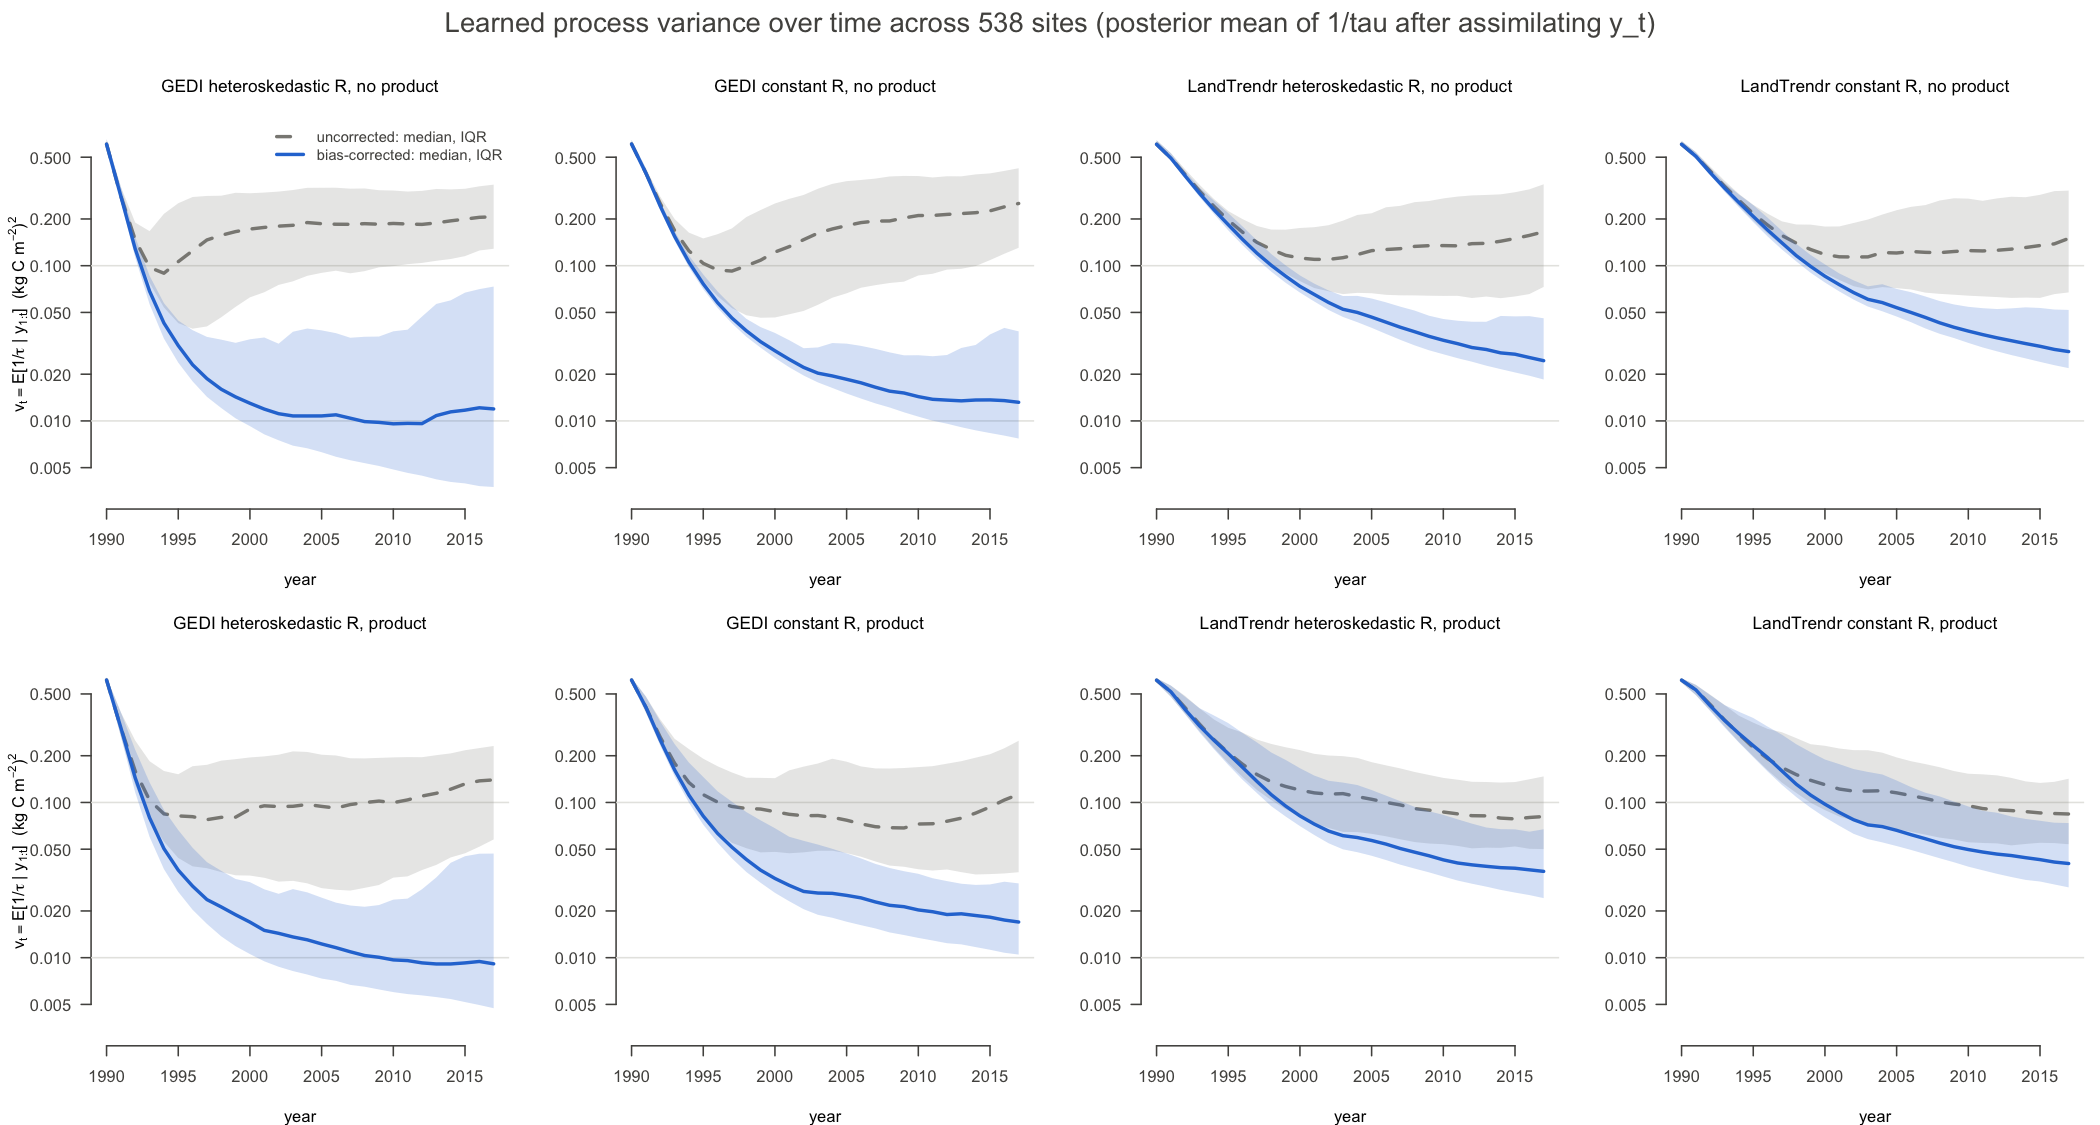
\includegraphics[width=\textwidth]{fw_procvar_time.png}
  \caption{Learned process variance $v_t = \E[1/\tau \mid y_{1:t}]$ over time (log scale).
  Lines are the median over 538 sites and bands the IQR. Gray dashed: uncorrected;
  blue: bias-corrected. Rows: without and with the disturbance product.}
  \label{fig:procvar}
\end{figure}

\begin{table}[ht]
  \centering\small
  \begin{tabular}{lrrrrrr}
    \toprule
    & \multicolumn{2}{c}{median $v_t$, 1995} & \multicolumn{2}{c}{median $v_T$, 2017} & median & sites with \\
    experiment & uncorr. & corr. & uncorr. & corr. & $v_T^{\rm corr}/v_T^{\rm uncorr}$ & smaller $v_T$ \\
    \midrule
    GEDI het., no product        & 0.106 & 0.031 & 0.207  & 0.0119  & 0.08 & 94\% \\
    GEDI const., no product      & 0.103 & 0.076 & 0.252  & 0.0132  & 0.07 & 92\% \\
    LandTrendr het., no product  & 0.196 & 0.184 & 0.165  & 0.0244  & 0.18 & 87\% \\
    LandTrendr const., no product& 0.216 & 0.208 & 0.150  & 0.0280  & 0.22 & 86\% \\
    GEDI het., product           & 0.082 & 0.037 & 0.140  & 0.0091  & 0.15 & 92\% \\
    GEDI const., product         & 0.112 & 0.082 & 0.113  & 0.0170  & 0.22 & 86\% \\
    LandTrendr het., product     & 0.209 & 0.206 & 0.081  & 0.0360  & 0.58 & 75\% \\
    LandTrendr const., product   & 0.226 & 0.232 & 0.084  & 0.0404  & 0.57 & 75\% \\
    \bottomrule
  \end{tabular}
  \caption{Learned process variance $v_t$ ((kg\,C\,m$^{-2}$)$^2$) in 1995 and 2017, and the
  per-site ratio of corrected to uncorrected $v_T$.}
  \label{tab:procvar}
\end{table}

You expected the process variance learned with bias correction to be smaller. It is, by a lot
(Table~\ref{tab:procvar}).

\begin{itemize}
  \item \textbf{Without correction, the process variance absorbs the bias.} In the GEDI experiments without the product (and, more weakly, GEDI heteroskedastic $R$ with it) the
  uncorrected $v_t$ falls until about 1995 and then \emph{rises}, to about 0.2 by 2017. The forecast
  errors there have a consistent sign (VSEM over-predicts wood). The only way the
  uncorrected filter can account for errors that large is a larger process variance, so the
  $\tau$ posterior moves to smaller $\tau$. With correction, the systematic part is removed
  and $v_t$ keeps falling, to about 0.01, a process standard deviation of about 0.1\,kg\,C\,m$^{-2}$\,yr$^{-1}$.
  \item \textbf{With LandTrendr error, the two curves agree until about 2000.} With $R \approx 3$--4 each observation says little about
  $\tau$, so $v_t$ falls slowly and the bias only starts to matter after several years of
  data. The corrected curve still ends 5--7 times lower (without the product).
  \item \textbf{The product shrinks the effect.} In flagged years the predictive includes the disturbance
  components, and the filter can explain a low observation as a disturbance instead of
  through $\tau$. The uncorrected $v_t$ is therefore smaller with the product, and the gap to the
  corrected run is smaller too.
  \item \textbf{The $\tau$ grid limit is not binding.} The smallest process variance on the grid is
  $1/\tau_{\max} = 10^{-4}$, and no site has $v_T < 10^{-3}$ in any experiment. The
  posterior is not stuck at the edge of the grid.
\end{itemize}

So the process variance is not why the corrected forecast is too wide: it is already
small and became smaller with correction.

%================================================================================
\section{Variance budget of the predictive}
\label{sec:budget}

\begin{figure}[ht]
  \centering
  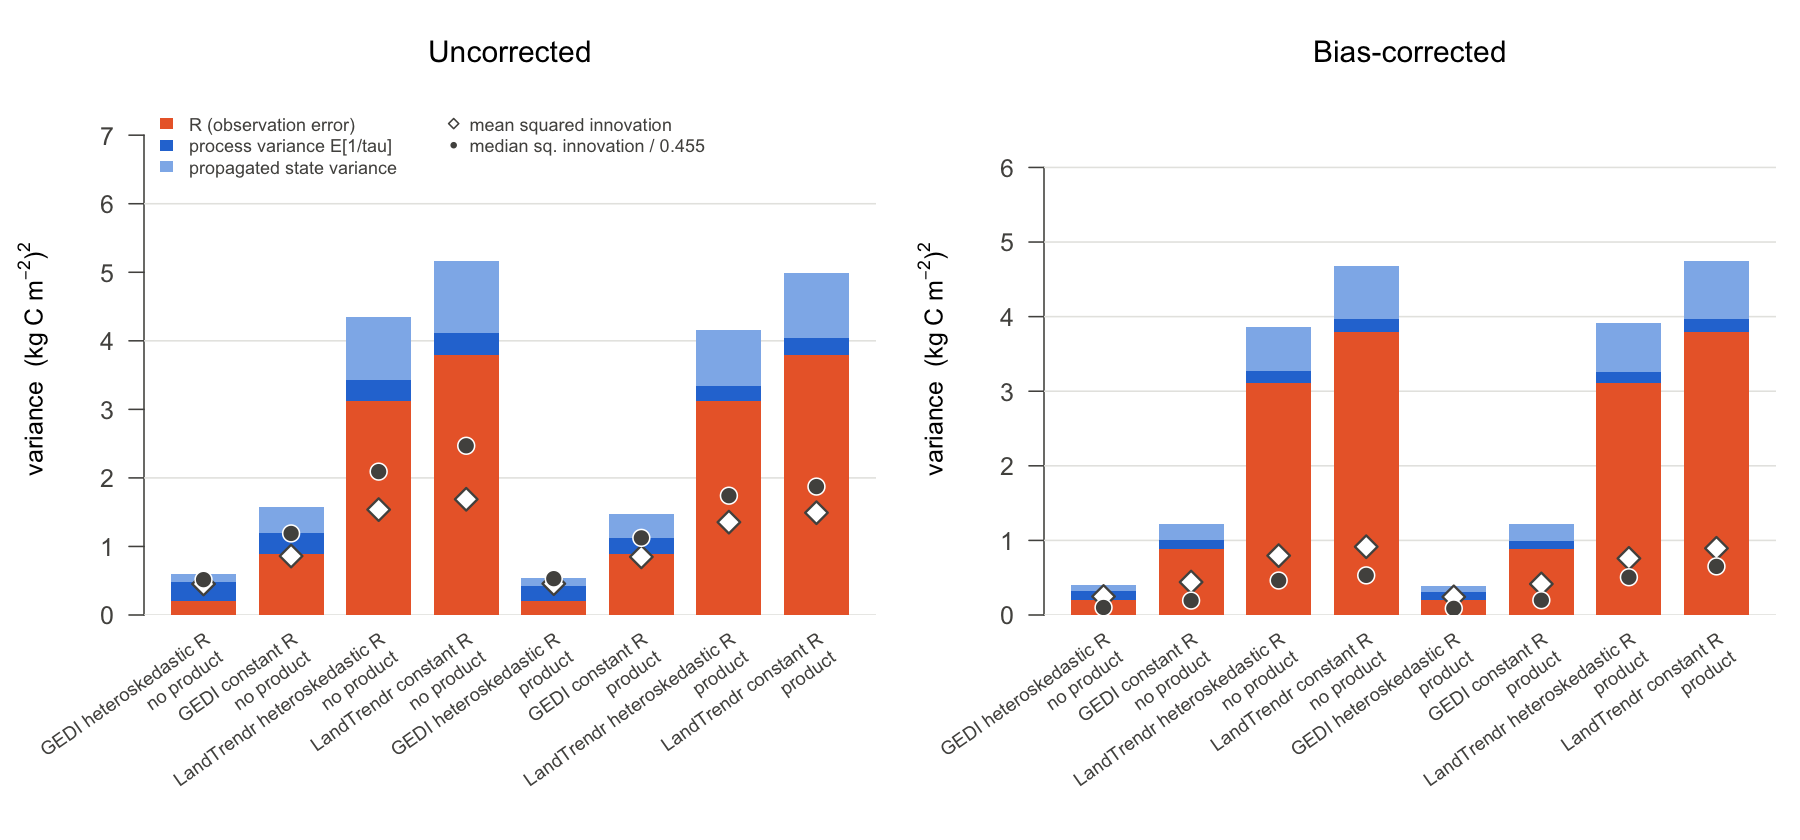
\includegraphics[width=\textwidth]{fw_variance_budget.png}
  \caption{Mean variance budget $\bar V^0 = \bar R + \bar Q + \bar P$ of the no-disturbance
  predictive over undisturbed site-years (100-site subset), against the mean squared
  innovation $\overline{e^2}$ (diamonds) and the median squared innovation divided by 0.455
  (dots; the median of $e^2$ is $0.455\,\Var(e)$ for Gaussian $e$). The predictive is
  calibrated when the bar height equals the markers.}
  \label{fig:budget}
\end{figure}

\begin{table}[ht]
  \centering\small
  \begin{tabular}{lcrrrrrrrrr}
    \toprule
    experiment (no product) & corr. & $\overline{e^2}$ & med $e^2$ & $\bar R$ & $\bar Q$ & $\bar P$ & $\bar V^0$ & $\E[z^2]$ & med $|z|$ & $c_R$ \\
    \midrule
    GEDI het.         & no  & 0.452 & 0.235 & 0.201 & 0.284 & 0.115 & 0.600 & 0.81 & 0.68 & 0.27 \\
                      & yes & 0.248 & 0.046 & 0.201 & 0.124 & 0.072 & 0.398 & 0.65 & 0.39 & 0.26 \\
    GEDI const.       & no  & 0.860 & 0.541 & 0.885 & 0.318 & 0.368 & 1.570 & 0.57 & 0.60 & 0.20 \\
                      & yes & 0.441 & 0.088 & 0.885 & 0.124 & 0.213 & 1.220 & 0.35 & 0.28 & 0.12 \\
    LandTrendr het.   & no  & 1.540 & 0.952 & 3.120 & 0.312 & 0.914 & 4.340 & 0.35 & 0.48 & 0.10 \\
                      & yes & 0.796 & 0.210 & 3.120 & 0.150 & 0.598 & 3.860 & 0.20 & 0.23 & 0.02 \\
    LandTrendr const. & no  & 1.690 & 1.120 & 3.800 & 0.314 & 1.050 & 5.160 & 0.32 & 0.47 & 0.09 \\
                      & yes & 0.915 & 0.242 & 3.800 & 0.164 & 0.708 & 4.670 & 0.19 & 0.23 & 0.01 \\
    \bottomrule
  \end{tabular}
  \caption{Variance budget of the no-disturbance predictive over undisturbed site-years
  (about 1840 per row), in (kg\,C\,m$^{-2}$)$^2$. Calibrated values: $\E[z^2] = 1$,
  median $|z| = 0.674$, $c_R = 1$. The runs with the product give nearly the same
  numbers; for LandTrendr, $c_R$ is slightly negative with the product (the $Q$ and $P$ parts alone
  exceed $\overline{e^2}$).}
  \label{tab:budget}
\end{table}

\begin{figure}[ht]
  \centering
  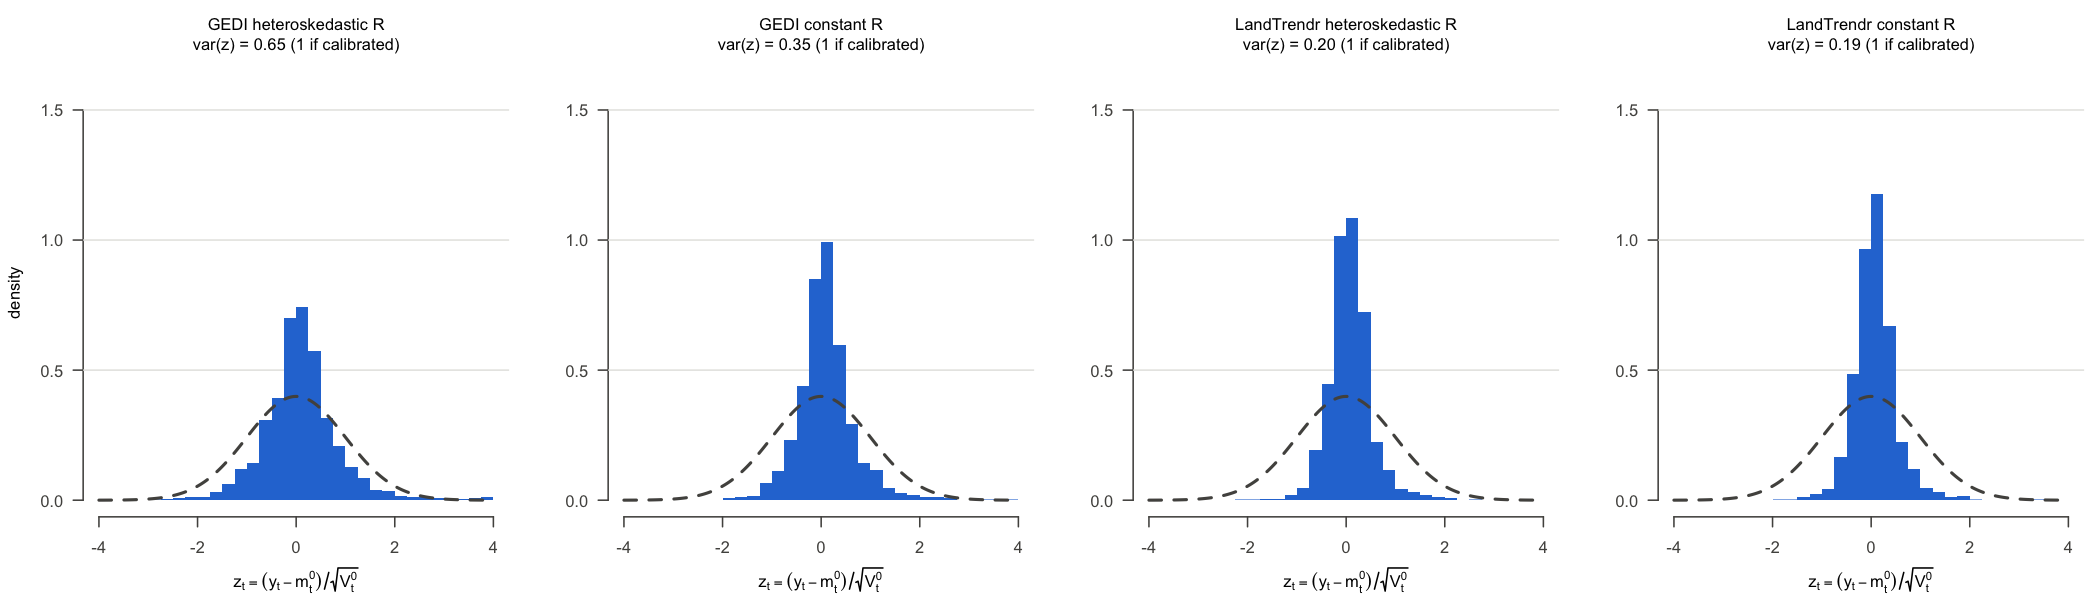
\includegraphics[width=\textwidth]{fw_std_innov.png}
  \caption{Standardised innovations $z_t = (y_t - m^0_t)/\sqrt{V^0_t}$ of the bias-corrected
  runs without the product, over undisturbed site-years. Dashed: $\Norm(0,1)$, the
  calibrated reference.}
  \label{fig:z}
\end{figure}

Table~\ref{tab:budget} and Figures~\ref{fig:budget}--\ref{fig:z} show where the predictive
width comes from.

\begin{itemize}
  \item \textbf{The correction reduces the errors more than the width.} For GEDI heteroskedastic $R$, the mean squared
  innovation halves (0.45 to 0.25) and the process part $Q$ falls from 0.28 to 0.12.
  But $R = 0.20$ stays in the predictive regardless, so $V^0$ falls only from 0.60 to 0.40. As a result $\E[z^2]$
  \emph{drops} from 0.81 to 0.65: relative to its errors, the corrected predictive is more too wide
  than the uncorrected one. The same holds in every experiment. This is why the corrected
  PIT histograms are more humped than you might expect. Before correction, the bias inflated the
  errors enough to roughly match the wide predictive.
  \item \textbf{$R$ alone is too large.} For GEDI constant $R$ and both LandTrendr settings, $\bar R$ is larger than
  the whole mean squared innovation (0.885 vs 0.44, 3.12 vs 0.80, 3.80 vs 0.92). Even with
  zero process variance and perfect knowledge of the state, the predictive would be too wide.
  To match the mean squared innovation, $R$ would have to be scaled by $c_R \approx 0.26$
  (GEDI heteroskedastic), $0.12$ (GEDI constant) and $0.01$--$0.02$ (LandTrendr).
  \item \textbf{$R$ also widens the predictive through $P$.} For a scalar Kalman update, the analysis
  variance is $P^a = P^f R/(P^f + R)$. When $R \gg P^f$, $P^a \approx P^f$: the
  observation barely reduces the state uncertainty, and that uncertainty is carried into the
  next forecast. The propagated part is $\bar P \approx 0.07$ for GEDI heteroskedastic and 0.6--0.7
  for LandTrendr. So a large $R$ widens the predictive twice: directly, and through a poorly constrained
  state.
  \item \textbf{The innovations are heavy-tailed.} For a Gaussian, the median of $e^2$ is $0.455\,\E[e^2]$. For the
  corrected runs it is $0.18$--$0.26\,\E[e^2]$: most years have very small
  errors and a few have large ones. Even for GEDI heteroskedastic, where the average variance is
  closest to calibrated ($\E[z^2] = 0.65$), the typical $|z|$ is 0.39 against 0.674, and 97\% of $|z|$
  fall within $\pm 1.96$ (expected 95\%). A Gaussian predictive with the right variance is still too
  wide in typical years and too narrow in jump years (Figure~\ref{fig:z}).
  \item \textbf{The disturbance tail adds width but not the hump.} The disturbed components add about
  1.1--1.25 to the full predictive variance ($V_t - V^0_t$) in every experiment. That variance sits in
  a low tail holding only the background disturbance probability (about 5\% per
  year). It moves the PIT of an undisturbed year by about that 5\%, but it is not what makes the
  hump, which already appears in $z_t$ (Figure~\ref{fig:z}).
\end{itemize}

%================================================================================
\section{Why $R$ is too large: the observations are smooth in time}
\label{sec:dy}

\begin{figure}[ht]
  \centering
  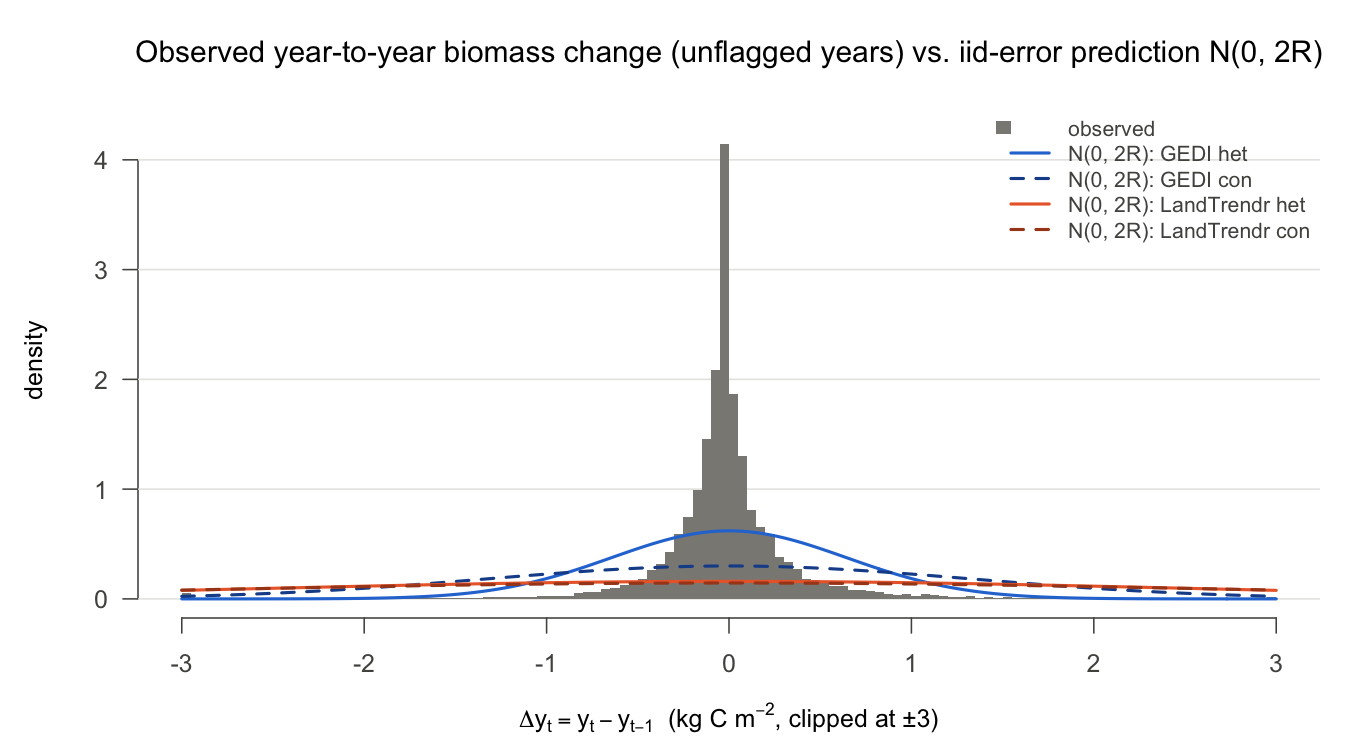
\includegraphics[width=0.85\textwidth]{fw_obs_change.png}
  \caption{Histogram of the observed year-to-year change $\Delta y_t$ over 10\,720 pairs of
  consecutive years not flagged by the product (538 sites), against $\Norm(0, 2\bar R)$, the smallest
  spread that independent observation errors with variance $R$ allow, for each observation-error
  model.}
  \label{fig:dy}
\end{figure}

This section uses only the data, not the filter. Suppose $y_t = x_{t,3} + \epsilon_t$ with independent
$\epsilon_t$ of variance $R_t$. Then
\[
  \Var(\Delta y_t) = \Var(\Delta x_{t,3}) + R_t + R_{t-1} \ \ge\ R_t + R_{t-1}.
\]
Now allow the errors to be correlated, with lag-1 correlation $\rho$ and equal variance $R$. Then
$\Var(\Delta \epsilon_t) = 2R(1-\rho)$, so
$\rho \ge \rho_{\min} = 1 - \Var(\Delta y)/(2\bar R)$.

\begin{table}[ht]
  \centering\small
  \begin{tabular}{lrrrr}
    \toprule
    observation-error model & $2\bar R$ & $\Var(\Delta y)/2\bar R$ & robust $\Var(\Delta y)/2\bar R$ & $\rho_{\min}$ \\
    \midrule
    GEDI heteroskedastic       & 0.414 & 0.70  & 0.117  & 0.88 \\
    GEDI constant              & 1.770 & 0.16  & 0.027  & 0.97 \\
    LandTrendr heteroskedastic & 6.240 & 0.046 & 0.0077 & 0.99 \\
    LandTrendr constant        & 7.600 & 0.038 & 0.0064 & 0.99 \\
    \bottomrule
  \end{tabular}
  \caption{Observed year-to-year change against the lower bound $2\bar R$ implied by independent observation
  errors. $\Var(\Delta y) = 0.290$ and robust $\Var(\Delta y) = 0.048$ (kg\,C\,m$^{-2}$)$^2$, the same for every row.
  $\rho_{\min}$ uses the robust variance.}
  \label{tab:dy}
\end{table}

\begin{itemize}
  \item \textbf{The observed changes are far smaller than independent errors allow.} The robust variance of $\Delta y$
  is 12\% of $2\bar R$ for GEDI heteroskedastic and under 1\% for LandTrendr
  (Table~\ref{tab:dy}, Figure~\ref{fig:dy}). The median $|\Delta y|$ is 0.10\,kg\,C\,m$^{-2}$.
  \item \textbf{The series look smoothed.} 21\% of year-to-year changes are exactly zero, and the values come on a 0.05\,kg\,C\,m$^{-2}$ grid
  (1\,Mg\,ha$^{-1}$ of biomass). The changes are \emph{positively} correlated from one year to
  the next (lag-1 correlation $+0.32$). Independent errors would make it negative, since
  $\mathrm{Corr}(\Delta\epsilon_t, \Delta\epsilon_{t-1}) = -1/2$. This is what a
  temporally fitted product looks like (for example LandTrendr's piecewise-linear
  segmentation): the trajectory is smooth, and its error relative to the truth is persistent from year to
  year.
  \item \textbf{This explains the size of $c_R$.} With persistent errors, a site that is over-estimated one year is
  over-estimated the next. In the one-step innovation, most of $\epsilon_t$ is already
  explained by $\epsilon_{t-1}$, which the previous analysis partly absorbed into the state.
  For a first-order autoregressive (AR(1)) error, the part of $\epsilon_t$ that $\epsilon_{t-1}$ cannot predict
  has variance $R(1-\rho^2)$. At $\rho_{\min}$ this is $0.22R$ (GEDI heteroskedastic),
  $0.05R$ (GEDI constant) and $0.01$--$0.02R$ (LandTrendr), close to the scales $c_R$ the
  innovations ask for in Table~\ref{tab:budget} (0.26, 0.12, 0.01--0.02). The filter
  instead adds the full $R$ to every year's predictive variance.
  \item \textbf{Why the stated $R$ is not wrong as such.} The \code{Rparams} describe the error of a single biomass map
  relative to the truth, which is the right quantity for one snapshot. It is the wrong
  quantity for year-to-year innovations when that error persists over time.
  \item \textbf{The raw variance hides this.} The non-robust ratio for GEDI heteroskedastic is 0.70, much
  closer to 1, because a few large jumps (unflagged disturbances and product artefacts)
  dominate the plain variance. This is the same heavy tail seen in the innovations.
\end{itemize}

One consequence for the bias correction: $b_t$ estimates the persistent offset between the
observations and the undisturbed forecast. At a given site that offset is the VSEM bias
\emph{plus} the site's persistent observation error, and the filter cannot separate the two. The
correction therefore absorbs part of the persistent observation error, which helps the innovations.

%================================================================================
\section{Implications}

\begin{enumerate}
  \item \textbf{Use an innovation-scale observation error.} Replace $R$ in the filter with the variance of the
  non-persistent part, $R(1-\rho^2)$, with $\rho$ estimated per product, or estimate
  a scale $c$ on $R$ from the data. A scale can go on a grid jointly with $\tau$, using the same
  machinery as the $\tau$ posterior. The innovations point to $c \approx 0.1$--$0.3$ for GEDI and
  about 0.01--0.02 for LandTrendr.
  \item \textbf{Or model the persistence explicitly.} Add the observation-error offset to the state as an AR(1)
  term. The bias $b_t$ already works like a slowly updated version of this offset;
  modelling it would let the filter separate VSEM bias from observation offset over many
  sites.
  \item \textbf{Then handle the heavy tails.} After the scale is fixed, a Student-$t$ or two-component
  observation or process error would cover the rare jumps without widening every year.
  \item \textbf{Re-check the disturbance product's flags.} The second PIT peak near 0.8 (not analysed here)
  comes from flagged years without a visible biomass drop.
\end{enumerate}

%================================================================================
\section{Reproducing}

\begin{itemize}
  \item Code changes: \code{ORJointUpdate} now also returns \code{predMean0}, \code{predVar0}
  and \code{predProcVar0}, the no-disturbance predictive defined in Section~\ref{sec:pred0}.
  \item Uncorrected grid: \code{Rscript run\_grid.R} with \code{grid.outdir <- "experiments/fullRunNoBias"}
  and \code{grid.bias <- NULL} in the \code{run-grid} chunk.
  \item Figures and every number in this note:
  \code{Rscript claude-working-docs/forecast\_width\_analysis.R}, from the repository root
  (set \code{EXP\_DIR} if the experiment folders are elsewhere). The script reruns the
  100-site subset into \code{experiments/forecastWidth} if it is missing.
\end{itemize}

\end{document}
